\documentclass{uimppracticas}

%Permitir cabeceras y pie de páginas personalizados
\pagestyle{fancy}

%Path por defecto de las imágenes
\graphicspath{ {./images/} }

%Declarar formato de encabezado y pie de página de las páginas del documento
\fancypagestyle{doc}{
	%Pie de Página
	\footerpr{}{}{{\thepage} de \pageref{LastPage}}
}

%Declarar formato de encabezado y pie del título e indice
\fancypagestyle{titu}{%
	%Cabecera
	\headerpr{}{}{}
	%Pie de Página
	\footerpr{}{}{}
}

\appto\frontmatter{\pagestyle{titu}}
\appto\mainmatter{\pagestyle{doc}}

\begin{document}
	
%Comienzo formato título
\frontmatter

%Portada (Centrado todo)
\centeredtitle{./images/LogoUIMP.png}{Máster Universitario en Investigación en Inteligencia Artificial}{Curso 2020-2021}{Sistemas de Recomendación}{Recomendación para grupos \\ en Python}

\begin{center}
	\large \today
\end{center}

\vspace{40mm}

\begin{flushright}
	{\bf Laura Rodríguez Navas}\\
	\textbf{DNI:} 43630508Z\\
	\textbf{e-mail:} \href{rodrigueznavas@posgrado.uimp.es}{rodrigueznavas@posgrado.uimp.es}
\end{flushright}

\newpage

%Índice
\tableofcontents

\newpage

%Comienzo formato documento general
\mainmatter

\setlength\parskip{2.5ex}

\section{Introducción}\label{introducción}

El crecimiento de Internet y de la información disponible en línea ha hecho que sea mucho más difícil extraer información útil de manera efectiva. La abrumadora cantidad de datos requiere mecanismos de filtrado de información eficientes. Uno de los sistemas utilizados para hacer frente a este problema son los sistemas de recomendación.

En este documento se describe el desarrollo práctico en Python de un sistema de recomendación. El sistema de recomendación elegido se denomina de Filtrado Colaborativo (Usuario-Usuario). La implementación se puede encontrar en~\cite{GitHubRepo}, la cual está formada por el desarrollo de un programa que implementa el sistema de recomendación de \href{https://es.wikipedia.org/wiki/Filtrado_colaborativo}{Filtrado Colaborativo}. El documento se divide en diferentes secciones donde se va describiendo paso a paso el trabajo realizado. 

En la primera parte del documento se empieza describiendo la técnica de Filtrado Colaborativo, con sus ventajas y desventajas (ver secciones~\ref{filtro_colaborativo} y~\ref{ventajas_desventajas}). El documento sigue con la descripción del conjunto de datos que usa el sistema de recomendación, y cómo podemos adquirirlo (ver sección~\ref{conjunto_datos}).

En la sección~\ref{sistema_recomendacion} del documento se describe paso a paso la implementación en Python del sistema de recomendación de Filtrado Colaborativo. En esta sección también se describe el \href{https://es.wikipedia.org/wiki/Coeficiente_de_correlaci\%C3\%B3n_de_Pearson}{coeficiente de Correlación de Pearson} y porqué se ha elegido como medida para encontrar las similitudes entre los usuarios representados en el conjunto de datos y un nuevo usuario que he creado manualmente (ver sección~\ref{correlacion_pearson}). Además, también se aportan los resultados y su evaluación.

Finalmente, en la parte final del documento se añaden las conclusiones y la bibliografía.

\subsection{Filtrado Colaborativo}\label{filtro_colaborativo}

El Filtrado Colaborativo (FC) es una técnica utilizada por algunos sistemas de recomendación para predecir el grado en que, a un usuario U le gustaría un producto X. Esta técnica nos permite crear recomendaciones personalizadas, ayudar a los usuarios a encontrar productos de su interés, etc. analizando datos de muchos usuarios; asumiendo que los usuarios con gustos parecidos tienden a valorar los productos de forma similar. Es decir, si un usuario A tiene la misma opinión que un usuario B sobre un tema, el usuario A es más probable que tenga la misma opinión que el usuario B en otro tema diferente que la opinión que tendría un usuario elegido al azar. En resumen, el Filtrado Colaborativo es un método para hacer predicciones automáticas (filtrado) sobre los intereses de un usuario mediante la recopilación de las preferencias o gustos de información de muchos usuarios (colaboradores). 

Los sistemas de filtrado colaborativos basados en los usuarios, siguen una metodología que puede reducirse en los dos pasos siguientes:

\begin{itemize}
	\item En la búsqueda de usuarios que comparten los mismos patrones de valoración con el usuario activo (el usuario para el que se está haciendo la predicción).
	\item En utilizar las valoraciones por parte de aquellos usuarios afines que se encuentran en el paso 1 para calcular una predicción para el usuario activo.
\end{itemize}

En la sección~\ref{sistema_recomendacion} podremos ver detalladamente la metodología usada por el sistema de recomendación que se ha implementado en esta práctica.

\subsection{Ventajas y Desventajas del Filtrado Colaborativo}\label{ventajas_desventajas}

Algunas ventajas de un sistema de recomendación de Filtrado Colaborativo son:

\begin{itemize}
	\item Tiene en cuenta las valoraciones de otros usuarios.
	\item No necesita estudiar o extraer la información de los elementos recomendados.
	\item Se adapta a los intereses del usuario si estos cambian con el tiempo.
\end{itemize}

Algunas desventajas de un sistema de recomendación de Filtrado Colaborativo son:

\begin{itemize}
	\item Difícil de aplicar con grandes cantidades de usuarios.
	\item Difícil para encontrar suficientes vecinos para recomendar.
	\item Predice peor cuando existen pocas valoraciones.
	\item Difícil de aplicar cuando tenemos pocos datos de un nuevo producto (no ha sido valorado o ha sido poco valorado por los usuarios); o de un nuevo usuario (desconocemos sus valoraciones). Este problema se denomina el problema del \href{https://es.wikipedia.org/wiki/Arranque_en_fr\%C3\%ADo}{arranque frío}.
\end{itemize}

Para aliviar las desventajas se suele recurrir a sistemas de recomendación híbridos, que utilizan a la vez sistemas de recomendación de filtrado colaborativo y sistemas de recomendación basados en contenido. Los sistemas de recomendación basados en contenido son aquellos que tomando en cuenta algunos datos del historial del usuario intenta predecir que busca el usuario y que sugerencias similares puede mostrar. Este tipo de sistemas es uno de los que tiene mayor presencia en la actualidad.

En esta práctica no me ha parecido necesario el uso de un sistema de recomendación híbrido.

\section{Conjunto de datos}\label{conjunto_datos}

El conjunto de datos que se ha usado en esta práctica se encuentra disponible públicamente para su descarga en el siguiente enlace: \url{https://www.kaggle.com/abhikjha/movielens-100k/download}. Este conjunto de datos llamado \textit{ml-latest-small}, describe las valoraciones (entre 1 y 5 estrellas) y la actividad del etiquetado de \href{http://movielens.org}{MovieLens}~\cite{MovieLens}, un servicio de recomendación de películas. El conjunto de datos contiene 100836 valoraciones y 3683 etiquetas de 9742 películas. Los datos fueron creados por 610 usuarios que se seleccionaron al azar. Cada usuario clasificó al menos 20 películas diferentes y está representado por un identificador.

Una vez descargado el conjunto de datos podemos ver que está contenido en los archivos \textit{links.csv}, \textit{movies.csv}, \textit{ratings.csv} y \textit{tags.csv}. Aunque para esta práctica solo se utilizan los archivos \textit{movies.csv} y \textit{ratings.csv}, y estos se encuentran en la carpeta \textit{dataset} de~\cite{GitHubRepo}. Para mejorar las recomendaciones del sistema de recomendación, primero realizaremos un seguido de transformaciones en el conjunto de datos. Inicialmente empezamos cargando los archivos \textit{movies.csv} y \textit{ratings.csv} dentro de un dataframe (ver Definición~\ref{dataframe}) con el uso de la librería pandas~\cite{pandas}.

\begin{lstlisting}[language=python, basicstyle=\small]
movies_df = pd.read_csv('dataset/movies.csv')
ratings_df = pd.read_csv('dataset/ratings.csv')
\end{lstlisting}

Miramos el contenido de \textit{movies\_df} para ver cómo queda organizado:

\begin{table}[H]
	\centering
	\begin{tabular}{rll}
		\toprule
		movieId &                         title &                                       genres \\
		\midrule
		1 &                    Toy Story (1995) &  Adventure|Animation|Children|Comedy|Fantasy \\
		2 &                      Jumanji (1995) &                   Adventure|Children|Fantasy \\
		3 &             Grumpier Old Men (1995) &                               Comedy|Romance \\
		4 &            Waiting to Exhale (1995) &                         Comedy|Drama|Romance \\
		5 &  Father of the Bride Part II (1995) &                                       Comedy \\
		6 &                         Heat (1995) &                        Action|Crime|Thriller \\
		7 &                      Sabrina (1995) &                               Comedy|Romance \\
		8 &                 Tom and Huck (1995) &                           Adventure|Children \\
		9 &                 Sudden Death (1995) &                                       Action \\
		10 &                    GoldenEye (1995) &                    Action|Adventure|Thriller \\
		\bottomrule
	\end{tabular}
	\caption{Contenido del dataframe \textit{movies\_df} inicialmente.}
	\label{movies_df}
\end{table}

Cada película tiene un único identificador (\textit{movieId}), un título con su año de estreno y diferentes géneros. Como los años contienen caracteres \textit{unicode} y para que no haya problemas más adelante, los sacaremos de la columna de los títulos y los ubicaremos en su propia columna que nombraremos \textit{year}. Pues primero creamos una expresión regular para encontrar los años guardados entre paréntesis dentro de la columna de los títulos, y con la función \textit{extract} de la librería pandas los extraemos para guardarlos más adelante en su propia columna. Después borramos los años de la columna de los títulos con la función \textit{replace}, y finalmente, con la función \textit{strip} nos aseguramos de sacar los espacios extra que pudieran haber quedado durante este proceso de transformación. Además, eliminamos la columna de los géneros con la función \textit{drop}, ya que no la tendremos en cuenta en el sistema de recomendación.

\begin{lstlisting}[language=python, basicstyle=\small]
regular_expression = r'\((.*?)\)'
movies_df['year'] = movies_df.title.str.lower().str.extract(regular_expression)
movies_df['title'] = movies_df.title.str.replace(regular_expression, '', regex=True)
movies_df['title'] = movies_df['title'].apply(lambda x: x.strip())
movies_df = movies_df.drop('genres', 1)
\end{lstlisting}

Vemos el resultado:

\begin{table}[H]
	\centering
	\begin{tabular}{rll}
		\toprule
		movieId &                  title &  year \\
		\midrule
		1 &                    Toy Story &  1995 \\
		2 &                      Jumanji &  1995 \\
		3 &             Grumpier Old Men &  1995 \\
		4 &            Waiting to Exhale &  1995 \\
		5 &  Father of the Bride Part II &  1995 \\
		6 &                         Heat &  1995 \\
		7 &                      Sabrina &  1995 \\
		8 &                 Tom and Huck &  1995 \\
		9 &                 Sudden Death &  1995 \\
		10 &                    GoldenEye &  1995 \\
		\bottomrule
	\end{tabular}
	\caption{Contenido del dataframe \textit{movies\_df} final.}
	\label{movies_df_final}
\end{table}

\begin{definition}\label{dataframe}
	Un DataFrame es una estructura de datos bidimensional y etiquetada que acepta diferentes tipos datos de entrada organizados en columnas. Se puede pensar en un DataFrame como una hoja de cálculo o una tabla SQL.
\end{definition}

\newpage

Ahora, miraremos cómo está organizado el dataframe \textit{ratings\_df}. También le eliminamos una columna con la función \textit{drop}, la columna \textit{timestamp}, porqué tampoco se tendrá en cuenta en el sistema de recomendación.

\begin{lstlisting}[language=python, basicstyle=\small]
ratings_df = ratings_df.drop('timestamp', 1)
\end{lstlisting}

Así es cómo queda organizado el dataframe \textit{ratings\_df}:

\begin{table}[H]
	\centering
	\begin{tabular}{rrr}
		\toprule
		userId &  movieId &  rating \\
		\midrule
		1 &        1 &     4.0 \\
		1 &        3 &     4.0 \\
		1 &        6 &     4.0 \\
		1 &       47 &     5.0 \\
		1 &       50 &     5.0 \\
		1 &       70 &     3.0 \\
		1 &      101 &     5.0 \\
		1 &      110 &     4.0 \\
		1 &      151 &     5.0 \\
		1 &      157 &     5.0 \\
		\bottomrule
	\end{tabular}
	\caption{Contenido del dataframe \textit{ratings\_df}.}
	\label{ratings_df_final}
\end{table}

Cada fila del dataframe \textit{ratings\_df} tiene un identificador de usuario asociado con al menos una película y la valoración que ha realizado de ella. Por ejemplo, en la Tabla~\ref{ratings_df_final} vemos como el usuario 1 ha visto y valorado diferentes películas.

\section{Sistema de Recomendación}\label{sistema_recomendacion}

En esta sección describimos el sistema de recomendación, que como se ha comentado en la sección~\ref{filtro_colaborativo}, utiliza la técnica de Filtrado Colaborativo o también conocida como técnica de Filtrado de Usuario a Usuario. Con esta técnica el sistema de recomendación va a predecir recomendaciones de películas a un nuevo usuario acordes a sus gustos después de añadir nuevos datos al sistema. Para predecir las recomendaciones, el sistema de recomendación buscará las similitudes entre los datos introducidos por el nuevo usuario y los datos de los usuarios ya existentes en el sistema. Es decir, el sistema de recomendación intentará encontrar usuarios que tengan valoraciones parecidas a las del nuevo usuario, y entonces recomendarle al nuevo usuario películas acordes a sus valoraciones. Existen varios métodos para encontrar las similitudes entre los diferentes usuarios del sistema, y en el caso de este sistema, el método elegido se basa en el \href{https://es.wikipedia.org/wiki/Coeficiente_de_correlaci\%C3\%B3n_de_Pearson}{coeficiente de Correlación de Pearson} (ver sección~\ref{correlacion_pearson}).

El flujo de trabajo de este sistema de recomendación sigue estos pasos:

\begin{enumerate}
	\item Crea un nuevo usuario con las películas del conjunto de datos que el usuario a mirado.
	\item Basándose en el índice de selección de películas del nuevo usuario, encuentra a sus vecinos (usuarios similares a él).
	\item Obtiene los identificadores de las películas (movieId) donde el nuevo usuario y los vecinos coinciden, es decir, obtiene los identificadores de las películas que tanto el nuevo usuario como sus vecinos hayan visto.
	\item Calcula las similitudes entre el nuevo usuario y sus vecinos.
	\item Recomienda películas al nuevo usuario según las similitudes con sus vecinos.
\end{enumerate}

Así, siguiendo el flujo de trabajo anterior, comenzamos creando un nuevo usuario a quien recomendar películas. Para ello, hemos creado el archivo \textit{new\_user.csv} dentro de la carpeta \textit{dataset}, y le hemos añadido los títulos de 100 películas elegidas aleatoriamente del conjunto de datos con una nueva valoración. En este caso, he valorado las películas según mi criterio. Este archivo se puede modificar como se desee para realizar tantas recomendaciones como se quiera, solo debemos asegurarnos de escribir bien los títulos de las películas, igual que aparecen en el archivo \textit{dataset/movies.csv}, y que valoramos las películas con un valor entre 1 y 5. A continuación, visualizamos como se organiza parte del contenido del archivo \textit{new\_user.csv}:

\begin{figure}[H]
	\centering
	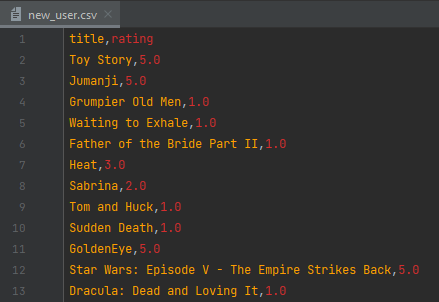
\includegraphics[scale=0.65]{images/new_user}
	\caption{Nuevo usuario del sistema.}
\end{figure}

Para finalizar con la creación del nuevo usuario, el archivo \textit{new\_user.csv} se carga dentro de un nuevo dataframe que llamaremos \textit{user\_df}.

\begin{lstlisting}[language=python, basicstyle=\small]
user_df = pd.read_csv('dataset/new_user.csv')
\end{lstlisting}

Con los datos del nuevo usuario en el conjunto de datos del sistema, extraemos los títulos de las películas que el usuario haya visto, guardándolos en la variable \textit{titles}, y los unimos a los datos del usuario almacenados en el dataframe \textit{user\_df}. En este punto para ahorrar un poco de espacio de memoria, aprovechamos a eliminar la columna \textit{year} del dataframe del nuevo usuario con la función \textit{drop}, ya que no se utilizará más adelante en el sistema de recomendación.

\begin{lstlisting}[language=python, basicstyle=\small]
titles = movies_df[movies_df['title'].isin(user_df['title'].tolist())]
user_df = pd.merge(titles, user_df)
user_df = user_df.drop('year', 1)
\end{lstlisting}

Así queda organizado el dataframe \textit{user\_df}:

\begin{table}[H]
	\centering
	\begin{tabular}{rlr}
		\toprule
		movieId &                  title &  rating \\
		\midrule
		1 &                    Toy Story &     5.0 \\
		2 &                      Jumanji &     5.0 \\
		3 &             Grumpier Old Men &     1.0 \\
		4 &            Waiting to Exhale &     1.0 \\
		5 &  Father of the Bride Part II &     1.0 \\
		6 &                         Heat &     3.0 \\
		7 &                      Sabrina &     2.0 \\
		915 &                      Sabrina &     2.0 \\
		8 &                 Tom and Huck &     1.0 \\
		9 &                 Sudden Death &     1.0 \\
		\bottomrule
	\end{tabular}
	\caption{Contenido del dataframe \textit{user\_df}.}
	\label{user_df}
\end{table}

Ahora que hemos añadido los identificadores de las películas con los datos del nuevo usuario, podemos obtener todos los usuarios que hayan visto las mismas películas (almacenados en \textit{movies}), que además agruparemos por su identificador de usuario (userId) con el método \textit{groupby}.

\begin{lstlisting}[language=python, basicstyle=\small]
movies = ratings_df[ratings_df['movieId'].isin(user_df['movieId'].tolist())]
users = movies.groupby(['userId'])
\end{lstlisting}

Por ejemplo, observamos los datos de uno de los usuarios, el usuario 525:

\begin{table}[H]
	\centering
	\begin{tabular}{rrr}
		\toprule
		userId &  movieId &  rating \\
		\midrule
		525 &        1 &     4.0 \\
		525 &        2 &     3.5 \\
		525 &       34 &     3.0 \\
		525 &       39 &     4.5 \\
		525 &       48 &     3.0 \\
		525 &       62 &     3.5 \\
		525 &      107 &     3.5 \\
		525 &      150 &     4.0 \\
		525 &      223 &     3.5 \\
		525 &      377 &     3.5 \\
		525 &      480 &     4.0 \\
		525 &      595 &     3.5 \\
		525 &      915 &     3.5 \\
		525 &     1196 &     4.5 \\
		\bottomrule
	\end{tabular}
	\caption{Películas que ha visto y valorado el usuario 525.}
	\label{user_525}
\end{table}

El usuario 525 en total ha valorado 14 películas, 12 de las cuales no han sido valoradas por el nuevo usuario del sistema (ver Tabla~\ref{user_df}). Este hecho podría entorpecer la predicción de las recomendaciones, así que, para una mejor recomendación, donde no será necesario pasar por todos los usuarios, ordenaremos el conjunto de datos de tal forma que los usuarios que compartan la mayor cantidad de películas tengan prioridad (usuarios comunes).

\begin{lstlisting}[language=python, basicstyle=\small]
common_users = sorted(users, key=lambda x: len(x[1]), reverse=True)
\end{lstlisting}

\subsection{Coeficiente de Correlación de Pearson}\label{correlacion_pearson}

Una vez encontrados los usuarios más comunes o similares del conjunto de datos, ya podemos medir la similitud entre ellos para predecir las recomendaciones. El sistema de recomendación buscará correlaciones entre patrones de valoración sobre las películas que han valorado los usuarios, viendo cómo se relacionan entre sí. Es decir, el sistema buscará las similitudes entre los usuarios y el nuevo usuario para encontrar aquellos que se parecen más a este. Para ello usaremos el \href{https://es.wikipedia.org/wiki/Coeficiente_de_correlaci\%C3\%B3n_de_Pearson}{coeficiente de Correlación de Pearson}. La fórmula para calcular este coeficiente sobre un estadístico muestral (vef Definición~\ref{estadístico_muestral}) se puede ver a continuación:

\begin{equation}\label{formula}
	\large r = \frac{\sum_{1}^{n} \; (x_{i} - \bar{x}) (y_{i} - \bar{y})}{\sqrt{\sum_{1}^{n}(x_{i} - \bar{x})^2} \; \sqrt{\sum_{1}^{n}(y_{i} - \bar{y})^2}}
\end{equation}

Los valores dados por la fórmula (\ref{formula}) pueden variar entre [-1,1].

\begin{itemize}
	\item Si $r=1$ (correlación positiva perfecta), entonces las valoraciones estarán perfectamente correlacionadas. Los usuarios tendrán los mismos gustos.
	\item Si $0<r<1$, entonces existe una correlación positiva. Los usuarios tendrán gustos parecidos.
	\item Si $-1<r<0$, entonces existe una correlación negativa. Los usuarios tendrán pocos gustos parecidos.
	\item Si $r=-1$ (correlación negativa perfecta), entonces las valoraciones estarán inversamente correlacionadas. Los usuarios no tendrán los mismos gustos.
\end{itemize}

Se ha decidido usar el coeficiente de Correlación de Pearson por una de sus propiedades. Esta propiedad nos dice que, si se multiplican todos los elementos por una constante distinta a cero o si se agrega cualquier constante a todos los elementos del coeficiente, este no cambiará con la escala. Por ejemplo, si tenemos dos vectores $X$ e $Y$, entonces $pearson(X,Y) = pearson(X,2\cdot Y+3)$. Esta es una propiedad muy importante en los sistemas de recomendación porqué si dos usuarios valoran dos elementos de manera completamente diferente, pero son usuarios muy parecidos (con gustos similares) contaríamos con valoraciones muy parecidas en escalas variadas y esto crearía grandes problemas en la predicción de las recomendaciones. El coeficiente de Correlación de Pearson es la medida más utilizada cuando hay variaciones entre magnitudes y escala en las valoraciones, aunque pudiéramos obtener valores altos de correlación si existen pocos usuarios con valoraciones en común.

\begin{definition}\label{estadístico_muestral}
En estadística un estadístico muestral es una medida cuantitativa, derivada de un conjunto de datos de una muestra, con el objetivo de estimar o inferir características de una población o modelo estadístico.
\end{definition}

A continuación, mostramos el código para calcular los coeficientes de Correlación Pearson. Los coeficientes los almacenaremos en el diccionario \textit{pearsonCorrelationDict}, donde las claves serán los identificadores de los usuarios y los valores de cada clave serán los coeficientes. Elegimos un subconjunto de usuarios (\textit{usersSubset}) para hacer las iteraciones, para no añadir demasiado sobrecoste computacional pasando por cada usuario.

\begin{lstlisting}[language=python, basicstyle=\small]
usersSubset = common_users[0:100]	
pearsonCorrelationDict = {}

for id, group in usersSubset:
	# The current user and the new user are ordered in the same way
	user = group.sort_values(by='movieId')
	movies = user_df.sort_values(by='movieId')
	
	# Number of ratings for user
	nRatings = len(user)
	
	# Common ratings of the current user with the new user
	temp_df = movies[movies['movieId'].isin(user['movieId'].tolist())]
	tempRatingList = temp_df['rating'].tolist()
	
	# Ratings of the current user
	tempUserList = user['rating'].tolist()
	
	# Calculate the Pearson Correlation between the current user and new user
	Uxx = sum([i ** 2 for i in tempRatingList])-pow(sum(tempRatingList), 2) / float(nRatings)
	Uyy = sum([i ** 2 for i in tempUserList])-pow(sum(tempUserList), 2) / float(nRatings)
	Uxy = sum(i * j for i, j in zip(tempRatingList, tempUserList))-sum(tempRatingList) * sum(tempUserList) / float(nRatings)
	
	# If the denominator is nonzero, then we divide, otherwise the correlation is 0
	if Uxx != 0 and Uyy != 0:
		pearsonCorrelationDict[id] = Uxy / sqrt(Uxx * Uyy)
	else:
		pearsonCorrelationDict[id] = 0
\end{lstlisting}

Inicialmente en cada iteración, se ordenan los datos de cada usuario instanciado y los datos del nuevo usuario de la misma manera, para que los valores no se mezclen más adelante. Después se obtiene el número de valoraciones del usuario instanciado y se obtienen las valoraciones en común de este con el nuevo usuario, y todo se almacena en una lista temporal llamada \textit{tempRatingList}. Guardamos también en una lista temporal las valoraciones del usuario instanciado (\textit{tempUserList}). Esto lo hacemos porqué siempre es mucho más fácil recorrer una lista que un dataframe. A continuación, calculamos el coeficiente de correlación de Pearson de cada usuario instanciado con el nuevo usuario basándonos en la fórmula (\ref{formula}), siempre comprobando que el dominador sea diferente a cero, sino el valor del coeficiente será 0.

Veamos como resultado el contenido del diccionario \textit{pearsonCorrelationDict}:

\begin{lstlisting}[language=bash, basicstyle=\small]
dict_items([(414, 0.1710335374313876), (599, 0.40123525382704545), (6, 0.20329349941761546), (474, 0.21044663004441924), (274, 0.3530769675354643), (68, 0.33059489678211385), (608, 0.3260682075724168), (182, -0.23109387695394956), (19, 0.3133595303614617), (307, -0.18843150346003273), (91, 0.31180055592445977), (314, -0.1855577860558229), (380, 0.45012727283065757), (84, 0.012277750762966397), (117, -0.06953551887224728), (480, 0.16458728710301657), (217, 0.3252127201443157), (483, -0.16673896789941262), (372, 0.05020839625891806), (470, 0.32705689114535186), (489, -0.025392998342644958), (600, 0.042693983860009506), (240, 0.05131981034870924), (337, 0.3214285714285713), (448, 0.3145474121592105), (559, 0.17567351114860863), (602, -0.01953661662911384), (603, -0.12466125165644129), (604, -0.11070047639148746), (226, -0.08878401871687391), (43, -0.4295675016629953), (57, 0.05739773181955021), (160, -0.23053561726821561), (181, -0.025450425803285343), (411, 0.4184472097595221), (492, 0.009531160645787254), (524, 0.554930806561758), (45, 0.38256520195621246), (58, 0.06698696164390111), (109, -0.08767933833518694), (288, 0.040138052643118996), (304, -0.05079155413724917), (438, 0.1689463508123878), (592, 0.06429719695335717), (597, -0.04354691441125118), (40, -0.046609537669447546), (64, 0.027500104500595552), (446, -0.29551933110701833), (501, -0.021239769762143604), (590, 0.1779059797601214), (191, -0.5019578060538685), (219, 0.48620274802831803), (284, -0.00550473542118167), (353, 0.20638197410277853), (386, -0.1111123018786146), (140, -0.08363570955493667), (357, -0.009026976808426818), (373, -0.13235807087846027), (42, -0.010032434901514608), (136, -0.1711753075974906), (177, 0.1690569419933152), (179, 0.09896799408051585), (249, 0.25782317138405986), (330, -0.0750008147037369), (368, 0.2405974233356921), (437, 0.04624821484746095), (477, 0.31049173032627525), (594, 0.008390572815346994), (18, 0.019351013185103308), (103, -0.003498129001342704), (112, 0.38778864063592566), (385, 0.5296480205051889), (387, 0.43198485996958375), (425, 0.09288282368076137), (541, 0.25728140367086977), (566, 0.0679837639353997), (584, 0.573224999318389), (32, -0.04999999999999922), (235, -0.30774536098405614), (266, 0.177355756021643), (391, -0.3687156994355351), (428, -0.24008629652200658), (458, 0.0843349010400103), (469, 0.10400998543792594), (555, -0.006953000128056482), (570, 0.2575275846563296), (580, 0.31742024784266926), (94, 0.5774257546144353), (144, -0.25560087159134015), (294, 0.4777456720827587), (318, -0.40396888282756127), (323, 0.2786429232355919), (381, 0.07479684684631624), (453, 0.0), (486, 0.3959797974644654), (534, 0.23281019568466926), (588, -0.16115829864721526), (606, -0.4177121530460993), (82, 0.3263157894736842), (121, -0.1532100435348196)])
\end{lstlisting}

Guardamos el resultado para una mejor visualización en un nuevo dataframe que llamaremos \textit{pearson\_df}, donde la columna \textit{similarityIndex} contendrá los coeficientes de Correlación de Pearson de cada usuario representado por el identificador de la columna \textit{userId}.

\begin{lstlisting}[language=python, basicstyle=\small]
pearson_df = pd.DataFrame.from_dict(pearsonCorrelationDict, orient='index')
pearson_df.columns = ['similarityIndex']
pearson_df['userId'] = pearson_df.index
pearson_df.index = range(len(pearson_df))
\end{lstlisting}

\newpage

Así queda organizado el contenido del nuevo dataframe \textit{pearson\_df}:

\begin{table}[H]
	\centering
	\begin{tabular}{rr}
		\toprule
		similarityIndex &  userId \\
		\midrule
		0.171034 &     414 \\
		0.401235 &     599 \\
		0.203293 &       6 \\
		0.210447 &     474 \\
		0.353077 &     274 \\
		0.330595 &      68 \\
		0.326068 &     608 \\
		-0.231094 &     182 \\
		0.313360 &      19 \\
		-0.188432 &     307 \\
		\bottomrule
	\end{tabular}
	\caption{Contenido del dataframe \textit{pearson\_df}.}
\label{pearson_df}
\end{table}


\subsection{Predicción y Resultado}

Como tenemos ordenado el conjunto de datos de tal forma que los usuarios que comparten la mayor cantidad de películas tienen más prioridad, podemos realizar una selección del vecindario. La selección del vecindario o la selección de los $K$ vecinos más cercanos, es la aproximación más común para seleccionar los $K$ usuarios más comunes o similares. $K$ es el número de vecinos que vamos a seleccionar, en teoría cuantos más vecinos seleccionemos para nuestro vecindario, mejores recomendaciones va a predecir el sistema de recomendación para el nuevo usuario. Porqué aplicando una selección del vecindario conseguiremos penalizar aquellas situaciones donde el cálculo de la similitud entre los usuarios haya obtenido pocas valoraciones en común. En este caso, seleccionamos el valor de $K$ igual a 50. Los 50 usuarios seleccionados son ordenados por sus coeficientes de forma ascendente, así en las primeras posiciones tendremos los usuarios más parecidos al nuevo usuario.

\begin{lstlisting}[language=python, basicstyle=\small]
topUsers = pearson_df.sort_values(by='similarityIndex', ascending=False)[0:50]
\end{lstlisting}

Veamos los primeros 10 usuarios más parecidos al nuevo usuario, que en este caso como yo he valorado las películas según mi criterio, son los primeros 10 usuarios más parecidos a mí.

\begin{table}[h]
	\centering
	\begin{tabular}{rr}
		\toprule
		similarityIndex &  userId \\
		\midrule
		0.577426 &      94 \\
		0.573225 &     584 \\
		0.554931 &     524 \\
		0.529648 &     385 \\
		0.486203 &     219 \\
		0.477746 &     294 \\
		0.450127 &     380 \\
		0.431985 &     387 \\
		0.418447 &     411 \\
		0.401235 &     599 \\
		\bottomrule
	\end{tabular}
	\caption{Los 50 usuarios más similares.}
	\label{top_50}
\end{table}

Parece que mis gustos no son muy parecidos a los de los otros usuarios que forman el conjunto de datos. Los coeficientes de Correlación de Pearson resultantes que podemos observar en la Tabla~\ref{top_50} no son muy altos. Por ejemplo, el valor de similitud con el usuario más parecido a mí, el usuario 94, es igual a 0.577426. Aun así, vamos a recomendar películas al nuevo usuario, es decir, a mí misma.

Para calcular las recomendaciones tomaremos el promedio ponderado de las valoraciones de las películas utilizando los coeficientes de la Correlación de Pearson. Se ha elegido el promedio ponderado como medida de predicción porqué se considera fácil de calcular y suele funcionar bastante bien, aunque no tiene en cuenta el sesgo en las valoraciones de los usuarios si tienden a valorar alto o bajo. 

El promedio ponderado se calcula aplicando la siguiente fórmula:

\begin{equation}\label{promedio_ponderado}
	\large \hat{r}_{u,i} = \frac{1}{\sum_{a\in K}sim(u,a)} \sum_{a\in K }sim(u,a) r_{a,i}
\end{equation}

A fin de calcular el promedio ponderado en el sistema de recomendación, primero debemos unir las valoraciones de todas las películas del dataframe \textit{ratings\_df} con los usuarios más similares al nuevo usuario (\textit{topUsers}). Esto logra organizar un nuevo dataframe que llamamos \textit{topUsersRating}.

\begin{lstlisting}[language=python, basicstyle=\small]
topUsersRating = topUsers.merge(ratings_df, left_on='userId', right_on='userId', 
	how='inner')
\end{lstlisting}

Vemos como queda organizado el nuevo dataframe  \textit{topUsersRating}:

\begin{table}[H]
	\centering
	\begin{tabular}{rrrr}
		\toprule
		similarityIndex &  userId &  movieId &  rating \\
		\midrule
		0.577426 &      94 &        2 &     4.0 \\
		0.577426 &      94 &       10 &     3.0 \\
		0.577426 &      94 &       11 &     3.0 \\
		0.577426 &      94 &       17 &     1.0 \\
		0.577426 &      94 &       19 &     2.0 \\
		0.577426 &      94 &       21 &     3.0 \\
		0.577426 &      94 &       32 &     5.0 \\
		0.577426 &      94 &       34 &     4.0 \\
		0.577426 &      94 &       39 &     1.0 \\
		0.577426 &      94 &       44 &     1.0 \\
		\bottomrule
	\end{tabular}
	\caption{Union del dataframe \textit{ratings\_df} con los usuarios más similares.}
	\label{ratings_similares}
\end{table}

Ahora ya podemos calcular el promedio ponderado aplicando la fórmula (\ref{promedio_ponderado}). Se realiza sencillamente multiplicando las dos columnas del dataframe \textit{topUsersRating}, \textit{similarityIndex} y \textit{rating}; y guardando el resultado en una nueva columna: \textit{weightedRating}. Ver el resultado en la Tabla~\ref{weightedRating}.

\begin{lstlisting}[language=python, basicstyle=\small]
topUsersRating['weightedRating'] = topUsersRating['similarityIndex'] * topUsersRating['rating']
\end{lstlisting} 

Después se suman los valores de las columnas \textit{similarityIndex} y \textit{weightedRating}, y se agrupan por la columna \textit{movieId}. Por último, separamos el resultado en dos columnas: la columna \textit{sum\_similarityIndex} que representa la suma de los coeficientes de Correlación de Pearson, y la columna \textit{sum\_weightedRating} que representa la suma de las valoraciones de los usuarios por sus coeficientes. Ver el resultado en la Tabla~\ref{sums}.

\begin{lstlisting}[language=python, basicstyle=\small]
tempTopUsersRating = topUsersRating.groupby('movieId').sum()[['similarityIndex', 'weightedRating']]
tempTopUsersRating.columns = ['sum_similarityIndex', 'sum_weightedRating']
\end{lstlisting} 

\begin{table}[H]
	\centering
	\begin{tabular}{rrrrr}
		\toprule
		similarityIndex &  userId &  movieId &  rating &  weightedRating \\
		\midrule
		0.577426 &      94 &        2 &     4.0 &        2.309703 \\
		0.577426 &      94 &       10 &     3.0 &        1.732277 \\
		0.577426 &      94 &       11 &     3.0 &        1.732277 \\
		0.577426 &      94 &       17 &     1.0 &        0.577426 \\
		0.577426 &      94 &       19 &     2.0 &        1.154852 \\
		0.577426 &      94 &       21 &     3.0 &        1.732277 \\
		0.577426 &      94 &       32 &     5.0 &        2.887129 \\
		0.577426 &      94 &       34 &     4.0 &        2.309703 \\
		0.577426 &      94 &       39 &     1.0 &        0.577426 \\
		0.577426 &      94 &       44 &     1.0 &        0.577426 \\
		\bottomrule
	\end{tabular}
	\caption{Multiplicación de las columnas \textit{similarityIndex} y \textit{rating}.}
	\label{weightedRating}
\end{table}

\begin{table}[H]
	\centering
	\begin{tabular}{rr}
		\toprule
		sum\_similarityIndex &  sum\_weightedRating \\
		&                     \\
		\midrule
		11.302189 &           43.880774 \\
		9.326976 &           30.408888 \\
		4.882914 &           12.700033 \\
		0.621741 &            1.446775 \\
		2.796576 &            8.189528 \\
		8.893940 &           34.706954 \\
		3.739738 &           10.699062 \\
		0.727404 &            2.182212 \\
		1.353227 &            4.100684 \\
		11.269351 &           40.952455 \\
		\bottomrule
	\end{tabular}
	\caption{Las columnas \textit{sum\_weightedRating} y \textit{sum\_weightedRating}.}
	\label{sums}
\end{table}

A continuación, se crea un dataframe vacío llamado \textit{recommendation\_df} para almacenar el promedio ponderado en una nueva columna (\textit{weighted\_average\_score}) que al final se obtiene de la división del contenido de las columnas \textit{sum\_weightedRating} y \textit{sum\_weightedRating}. En la Tabla~\ref{promedio_ponderado_resultado} vemos como se organiza el promedio ponderado dentro del nuevo dataframe \textit{recommendation\_df}.

\begin{lstlisting}[language=python, basicstyle=\small]
recommendation_df = pd.DataFrame()
recommendation_df['weighted_average_score'] = tempTopUsersRating['sum_weightedRating']/tempTopUsersRating['sum_similarityIndex']
recommendation_df['movieId'] = tempTopUsersRating.index
\end{lstlisting}

\begin{table}[H]
	\centering
	\begin{tabular}{rr}
		\toprule
		weighted\_average\_score &  movieId \\
		&          \\
		\midrule
		3.882502 &        1 \\
		3.260316 &        2 \\
		2.600913 &        3 \\
		2.326975 &        4 \\
		2.928412 &        5 \\
		3.902315 &        6 \\
		2.860912 &        7 \\
		\bottomrule
	\end{tabular}
	\caption{Promedio ponderado.}
	\label{promedio_ponderado_resultado}
\end{table}

Finalmente, se ordenan los valores del promedio ponderado de forma ascendente para ver las primeras 10 películas del conjunto de datos que el sistema de recomendación predice al nuevo usuario, o sea a mí. Podemos observar estas recomendaciones en la Tabla~\ref{recomendaciones_finales}.

\begin{lstlisting}[language=python, basicstyle=\small]
recommendation_df = recommendation_df.sort_values(by='weighted_average_score', ascending=False)
recommendation_df = movies_df.loc[movies_df['movieId'].isin(recommendation_df.head(10)['movieId'].tolist())]
\end{lstlisting}

\begin{table}[H]
	\centering
	\begin{tabular}{rll}
		\toprule
		movieId &                         title &  year \\
		\midrule
		2295 &                   Impostors, The &  1998 \\
		7121 &                       Adam's Rib &  1949 \\
		74754 &                        Room, The &  2003 \\
		82744 &                           Faster &  2010 \\
		95149 &  Superman/Batman: Public Enemies &  2009 \\
		102084 &             Justice League: Doom &  2012 \\
		108795 &                     Wonder Woman &  2009 \\
		147376 &    Doctor Who: A Christmas Carol &  2010 \\
		172875 &                A Detective Story &  2003 \\
		173145 &   War for the Planet of the Apes &  2017 \\
		\bottomrule
	\end{tabular}
	\caption{Las 10 mejores recomendaciones para el nuevo usuario.}
	\label{recomendaciones_finales}
\end{table}


\section{Conclusiones}

Automatizar la creación del archivo \textit{dataset/user\_ratings.csv}.

El enlace al vídeo debéis incluirlo en la memoria. Trabajo práctico: la idea es que vayáis explicando el porqué de las decisiones que habéis tomado (qué me llevó a utilizar unos determinados hiperparámetros, por qué he utilizado esta manera de medir la calidad de la solución,...) y hagáis un razonamiento sobre los resultados obtenidos.

Ahora, calculemos el coeficiente de correlación de Pearson entre el nuevo usuario y el resto de los usuarios del conjunto de datos. El resultado lo vamos a almacenar en un diccionario, donde la clave es el identificador del usuario y el valor es el coeficiente.


Este estudio presenta una aproximación a la recomendación que muestra
noticias ordenadas según el interés de los usuarios, expresados mediante
visitas previas y los términos contenidos en dichos artículos, así como en sus
categorías.
Se han diseñado dos modelos probabilísticos basados en el Aspect Model.
Los resultados muestran que cuando se considera la clasificación de las
noticias al general el modelo, ayuda mejor al usuario a acceder a las mismas.
Esta propuesta es interesante y una alternativa competitiva en el contexto de
los modelos de recomendación de noticias.
El modelo Triadic es mejor que el Diadic cuando se combina con la cuenta de
números de accesos, términos y categorías.

\renewcommand{\refname}{Bibliografía}
\bibliographystyle{unsrt}
\bibliography{biblio}
	
\end{document}
